% !TEX root = main.tex

\section{限制可满足性问题}
在搜索问题中,状态表示是个黑箱,可以有多种多样的方法来表达。
但实际上我们可以有特定的状态表示方法来解决大量不同的问题,在这种情况下的搜索算法可以变得很高效。

限制可满足性问题(Constraint Satisfaction Problem, CSP)指每一个状态都可以用一组特征值向量表示的问题。
\begin{itemize}
	\item $k$个特征/变量的集合$V_1,\ldots,V_n$
	\item 每一个变量都有一个包含有限值的论域$\dom[V_i]$,如
	\[\text{height}=\{\text{short},\text{average},\text{tall}\}\]
	\item 一组限制条件$C_1,\ldots,C_m$
	\begin{itemize}
		\item 每个限制条件都有一个作用域(scope),表示作用在什么变量上,如$C(V_1,V_2,V_4)$
		\item 相当于一个布尔函数,从变量赋值到布尔值的映射,如
		\[C(V_1=a,V_2=b,V_4=c)=True\]
		\item 布尔函数可以以表形式给出,或以表达式形式给出,如$C(V_1,V_2,V_4)=(V_1=V_2+V_4)$
	\end{itemize}
	\item 一个状态可以通过给每一个变量赋值得到
\end{itemize}

CSP不关心到目标状态的移动步骤,而只关心是否存在这样一组变量满足目标。

\subsection{回溯(backtracking)搜索}
对每一个变量分别赋值,深搜方式,同时结合启发式函数,用于在每一步选择不同的赋值变量。
\begin{figure}[H]
\centering
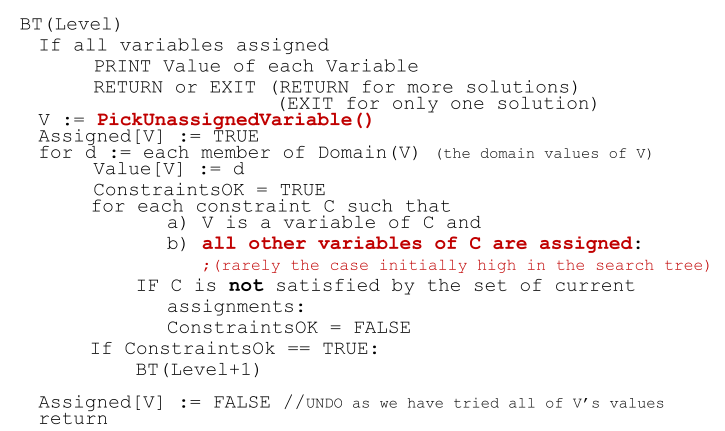
\includegraphics[width=0.6\linewidth]{fig/backtracking.png}
\end{figure}

回溯的问题在于不能提前探测到某一变量已经没有可以赋值了,导致依然要进入一层进行搜索。
因此考虑前瞻式算法,即限制传播(propagation)。
\begin{itemize}
	\item 甚至可以在还未进行搜索之前就采用
	\item 传播本身需要耗费资源,因此这里存在一个权衡
\end{itemize}

\subsection{向前检测}
\begin{enumerate}
	\item 选择一个未被赋值的变量$V$。这里可以采用最小剩余值(Minimum Remaining Values, MRV)作为启发式函数,即先选论域小的变量。
	\item 选择论域$\dom[V]$中的值对$V$进行赋值$d$
	\item 将$d$向前传递给含有$V$的限制$C$,主要考察那些\textbf{只剩一个未赋值变量$X$}的限制
	\item 检测\verb'FCCheck(C,X)'是否出现论域清空(Domain Wipe Out, DWO),即$X$没得选值了。
	这里\verb'FCCheck'做的则是核心的限制传播部分,当$V=d$后把$X$不能取的值删去
	\item 如果不出现DWO,则进入下一层(选择新的未赋值变量赋值)
	\item 否则需要恢复当层\verb'FCCheck'剪枝的部分,即$d$不可取,$V$要重新取值
\end{enumerate}
\begin{figure}[H]
\centering
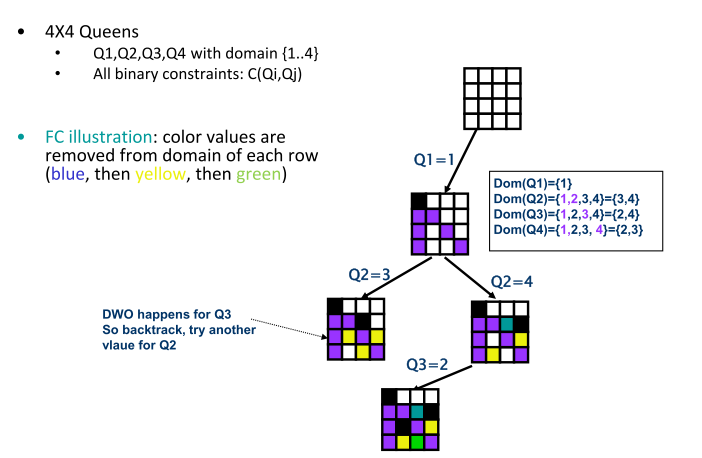
\includegraphics[width=0.6\linewidth]{fig/forward_checking_eg.png}
\end{figure}

\subsection{一般性边一致性(GAC)}
\begin{definition}[一致]
限制$C(X,Y)$是一致的,当且仅当对于所有$X$的值都存在某些$Y$满足$C$,即$\forall X\exists Y:\;C(X,Y)$。
\end{definition}
\begin{definition}[一般性边一致性(Generalized Arc Consistency, GAC)]
限制$C(V_1,V_2,\ldots,V_n)$是关于$V_i$边一致的,当且仅当$\forall V_i,\exists V_1,\ldots,V_{i-1},V_{i+1},\ldots,V_n$满足$C$。
限制$C$是GAC的当且仅当对于每一变量都是GAC的。
一个CSP是GAC的当且仅当它的限制都是GAC的。
\end{definition}

有GAC算法:
\begin{itemize}
\item 在$V_i=d$下,没有其他变量赋值能够满足该限制,则$d$是边不一致的,进而可以被剪枝剪掉。
\item 注意当从论域中移除一个值时可能导致新的不一致,故需要采用队列的方式,不断将需要检测边一致性限制添加,直到队列为空,即限制条件变为GAC。
\item 近似可理解为将后续搜索步骤都前移到剪枝部分。
\end{itemize}
\begin{figure}[H]
\centering
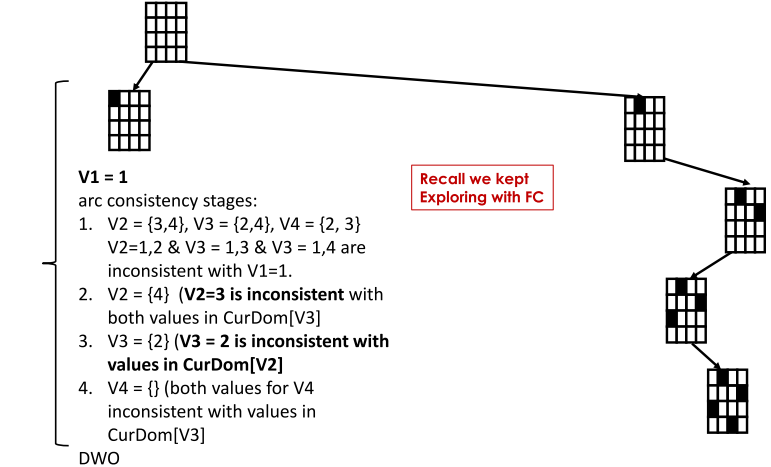
\includegraphics[width=0.6\linewidth]{fig/gac_eg.png}
\end{figure}

向前检测和边一致性检测的区别如下
\begin{figure}[H]
\centering
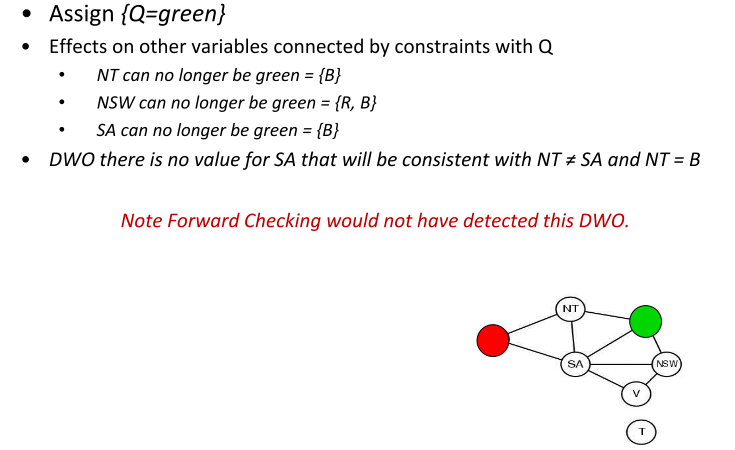
\includegraphics[width=0.8\linewidth]{fig/diff_fc_gac.png}
\end{figure}